% !TEX program = xelatex
\PassOptionsToPackage{table}{xcolor}
\documentclass[10pt, aspectratio=169]{beamer}

% --- 1. CẤU HÌNH & GÓI LỆNH ---
% VÌ SAO DÙNG FONTSPEC CHỨ KHÔNG DÙNG inputenc+T5:
%   Bản trước khai báo xelatex nhưng lại nạp inputenc + fontenc[T5] (setup của
%   pdflatex). Kết quả: PDF dùng font T5 "VnNimbusSansL", lớp text bị mất dấu —
%   pdftotext trả "Chờnh sòch" thay vì "Chính sách". XeLaTeX cần fontspec với
%   font Unicode thật để vừa hiển thị đúng vừa giữ được dấu khi copy/tìm kiếm.
\usepackage{fontspec}
\usepackage{polyglossia}
\setdefaultlanguage{vietnamese}
\setmainfont{Linux Libertine O}[
  BoldFont=Linux Libertine O Bold,
  ItalicFont=Linux Libertine O Italic
]
\setsansfont{Linux Biolinum O}[
  BoldFont=Linux Biolinum O Bold
]
\renewcommand{\familydefault}{\sfdefault}
\usepackage{booktabs}
\usepackage{tikz}
\usetikzlibrary{positioning}
\usepackage{pgf-pie}
\usepackage{amsmath}
\usepackage{graphicx}
\usepackage{subcaption}
\usepackage{multicol}
\usepackage{textpos}
\usepackage{ragged2e}
\usepackage{tabularx}
\usepackage{etoolbox}
\apptocmd{\frame}{}{\justifying}{}

\usepackage{caption}
\definecolor{captionlabelcolor}{RGB}{0,51,102}
\DeclareCaptionFont{captioncolor}{\color{black!95}}
\DeclareCaptionFont{labelcolor}{\color{captionlabelcolor}}
\captionsetup{
    font={small,bf,captioncolor},
    labelfont={bf,labelcolor},
    labelsep=period,
    justification=justified,
    singlelinecheck=false,
    textformat=period
}
\captionsetup[table]{
    font={small,bf,captioncolor},
    labelfont={bf,labelcolor},
    labelsep=period,
    justification=justified,
    singlelinecheck=false,
    name=BẢNG
}
\captionsetup[figure]{
    font={small,bf,captioncolor},
    labelfont={bf,labelcolor},
    labelsep=period,
    justification=justified,
    singlelinecheck=false,
    name=HÌNH
}

% --- 2. THEME & MÀU SẮC ---
\useinnertheme{circles}
\setbeamertemplate{navigation symbols}{}

% Màu sắc
\definecolor{HUEBlue}{RGB}{0, 51, 102}
\definecolor{HUEOrange}{RGB}{212, 175, 55}
\definecolor{HUEGreen}{RGB}{37, 139, 93}
\definecolor{DarkText}{RGB}{40, 40, 40}
\definecolor{LightGray}{RGB}{100, 100, 100}

\setbeamercolor{structure}{fg=HUEBlue}
\setbeamercolor{title}{fg=HUEBlue}
\setbeamercolor{frametitle}{fg=HUEBlue}
\setbeamercolor{section in head/foot}{bg=HUEBlue, fg=white}
\setbeamercolor{author in head/foot}{bg=HUEBlue!10, fg=HUEBlue}
\setbeamercolor{date in head/foot}{bg=HUEBlue!10, fg=HUEBlue}

% --- 3. GIAO DIỆN ---
\setbeamertemplate{headline}{
    \leavevmode
    \hbox{
        \begin{beamercolorbox}[wd=\paperwidth,ht=1.2cm,dp=0.5ex]{white}
            \hspace{0.3cm}
            \raisebox{0.2cm}{
\includegraphics[height=0.6cm, keepaspectratio]{logos/thpt_thuan_hoa}}
            \hfill
            \raisebox{0.2cm}{\color{LightGray}\tiny TRƯỜNG THPT THUẬN HÓA -- TRƯỜNG ĐẠI HỌC SƯ PHẠM, ĐẠI HỌC HUẾ}
            \hfill
            \raisebox{0.2cm}{
\includegraphics[height=0.6cm, keepaspectratio]{logos/dhsp_hue}}
            \hspace{0.3cm}
        \end{beamercolorbox}
    }
    \vskip0pt
    {\color{HUEOrange}\hrule height 2pt}
}

\setbeamerfont{frametitle}{size=\Large, series=\bfseries}
\setbeamertemplate{frametitle}{
    \vspace{0.2cm}
    \insertframetitle
    \par
    {\color{LightGray}\small \insertframesubtitle}
}

\setbeamercolor{block title}{fg=white, bg=HUEBlue}
\setbeamercolor{block body}{fg=DarkText, bg=HUEBlue!10}
\setbeamertemplate{blocks}[rounded][shadow=false]

% Mục lục chỉ xuất hiện ở slide 2; không chèn lại ở mỗi section để giữ giới hạn 15 slides.

% --- 4. THÔNG TIN ĐỀ TÀI ---
\title[AInatomy]{XÂY DỰNG PHÒNG THÍ NGHIỆM AI OFFLINE (AINATOMY) NHẰM PHÁT TRIỂN NĂNG LỰC KIỂM CHỨNG AI CHO HỌC SINH THPT THEO CHƯƠNG TRÌNH GIÁO DỤC PHỔ THÔNG 2018}
\subtitle{Báo cáo sản phẩm ứng dụng -- Giải thưởng Tiên phong Ứng dụng AI trong Giáo dục Việt Nam 2026}
\author[Mai Xuân Văn]{\textbf{Chủ trì:} Mai Xuân Văn\\
\textbf{Đơn vị:} Trường THPT Thuận Hóa, Đại học Sư Phạm, Đại học Huế}
\institute[THPT Thuận Hóa]{Trường THPT Thuận Hóa -- Đại học Sư Phạm, Đại học Huế}
\date{Năm học 2025--2026}

% ================= NỘI DUNG SLIDE =================
\begin{document}

% --- Slide 1: Trang bìa ---
\begin{frame}[plain]
    \centering
    \vspace{0.1cm}
    \begin{columns}
        \column{0.5\textwidth}
        \centering
        
\includegraphics[height=1.1cm, keepaspectratio]{logos/thpt_thuan_hoa}
        \column{0.5\textwidth}
        \centering
        
\includegraphics[height=1.1cm, keepaspectratio]{logos/dhsp_hue}
    \end{columns}
    \vspace{0.2cm}
    {\color{HUEOrange}\rule{0.8\textwidth}{2pt}}\\
    \vspace{0.3em}
    {\large \bfseries \color{HUEBlue} BÁO CÁO SẢN PHẨM ỨNG DỤNG} \\
    \vspace{0.5em}
    {\Large \bfseries \inserttitle} \\
    \vspace{0.3em}
    {\color{HUEOrange} \insertsubtitle} \\
    \vspace{0.4cm}
    \insertauthor \\
    \vspace{0.2cm}
    {\tiny \insertdate}
\end{frame}

% --- Slide 2: Mục lục ---
\begin{frame}{Cấu trúc báo cáo}
    \tableofcontents
\end{frame}

% ================= PHẦN 1: BỐI CẢNH VÀ VẤN ĐỀ =================
\section{Bối cảnh và vấn đề}

\begin{frame}{1.1. Bối cảnh giáo dục AI tại Việt Nam}
    \begin{columns}
        \column{0.6\textwidth}
        \textbf{Chính sách quốc gia:}
        \begin{itemize}
            \item Quyết định 2422/QĐ-BGDĐT (2024): 12 tiết/năm cho giáo dục AI trong THPT.
            \item Chương trình GDPT 2018: Tin học 10 có 22 yêu cầu cần đạt về AI.
        \end{itemize}
        \vspace{0.5em}
        \textbf{Thực trạng triển khai:}
        \begin{itemize}
            \item Phòng máy trường học yếu, internet không ổn định.
            \item Học sinh dễ dùng AI nhưng thiếu kỹ năng kiểm chứng đầu ra.
            \item Cần công cụ offline, không tài khoản, chạy được trên máy cấu hình thấp.
        \end{itemize}
        \column{0.4\textwidth}
        \begin{block}{Vấn đề cốt lõi}
            Làm thế nào để học sinh THPT \textbf{hiểu, kiểm tra và bắt lỗi AI} khi hạ tầng công nghệ hạn chế?
        \end{block}
    \end{columns}
\end{frame}

\begin{frame}{1.2. Ba thách thức cụ thể}
    \begin{alertblock}{1. Khó nhìn thấy AI}
        Dữ liệu, mô hình, thiên kiến và lỗi AI thường nằm ``bên trong'' hộp đen. Học sinh không thể quan sát cách AI hoạt động, chỉ thấy đầu ra cuối cùng.
    \end{alertblock}
    
    \vspace{0.3em}
    
    \begin{alertblock}{2. Khó triển khai thực tế}
        Phòng máy trường học có thể yếu hoặc mất mạng. Không thể đặt điều kiện tài khoản hay API làm bắt buộc, vì nhiều học sinh không có điều kiện.
    \end{alertblock}
    
    \vspace{0.3em}
    
    \begin{alertblock}{3. Khó kiểm chứng đầu ra}
        Học sinh dễ nhận đáp án từ AI mà chưa hình thành thói quen hỏi lại, kiểm tra độ tin cậy, và phát hiện lỗi — năng lực cốt lõi trong kỷ nguyên AI.
    \end{alertblock}
\end{frame}

% ================= PHẦN 2: GIẢI PHÁP VÀ CÔNG CỤ AI =================
\section{Giải pháp và công cụ AI}

\begin{frame}{2.1. Giải pháp: AInatomy}
    \begin{block}{Vấn đề cần giải quyết}
        Học sinh THPT cần học về AI theo chương trình mới, nhưng:
        \begin{itemize}
            \item Phòng máy trường học cấu hình thấp, internet không ổn định
            \item Không thể yêu cầu tài khoản hay kết nối API
            \item Cần công cụ trực quan để HS hiểu cách AI hoạt động
        \end{itemize}
    \end{block}
    
    \vspace{0.3em}
    
    \begin{block}{Giải pháp: AInatomy}
        \begin{itemize}
            \item \textbf{Offline 100\%:} Chạy trên máy RAM 2GB, không cần internet
            \item \textbf{Trực quan:} Mô phỏng 3D quy trình AI bằng Three.js
            \item \textbf{Tương tác:} HS tự tạo dữ liệu, huấn luyện mô hình, kiểm chứng kết quả
            \item \textbf{Bám sát chương trình:} Phủ 22 YCCĐ Tin học 10
        \end{itemize}
    \end{block}
    
    \vspace{0.3em}
    
    \begin{center}
        \textbf{Kết quả:} Học sinh hiểu AI từ bên trong, không chỉ sử dụng bên ngoài
    \end{center}
\end{frame}

\begin{frame}{2.2. Bốn bước học tập với AInatomy}
    \begin{enumerate}
        \item \textbf{Đọc:} Học sinh đọc tình huống, nhận diện vấn đề.
        \item \textbf{Dự đoán:} Học sinh dự đoán đầu ra AI trước khi xem kết quả.
        \item \textbf{Thực hiện:} Học sinh chạy mô phỏng AI, quan sát quy trình.
        \item \textbf{Phản hồi:} Học sinh so sánh dự đoán với kết quả, rút ra bài học.
    \end{enumerate}
    
    \vspace{0.5em}
    
    \begin{block}{Công cụ AI sử dụng}
        \begin{itemize}
            \item \textbf{Three.js:} Mô phỏng 3D quy trình AI (thu thập dữ liệu, huấn luyện, triển khai, đánh giá).
            \item \textbf{JavaScript:} Logic xử lý và tương tác người dùng.
            \item \textbf{HTML5/CSS3:} Giao diện responsive, hoạt động trên mọi trình duyệt.
        \end{itemize}
    \end{block}
\end{frame}

\begin{frame}{2.3. Bảy trạm trong Nhà máy AI}
    \begin{columns}
        \column{0.32\textwidth}
        \begin{block}{Trạm 0-2: Dữ liệu}
            \begin{itemize}
                \item \textbf{Trạm 0 — Nhập liệu:} Slider nội suy mượt (0-100\%)
                \item \textbf{Trạm 1 — Dán nhãn:} Học sinh tự dán nhãn
                \item \textbf{Trạm 2 — Huấn luyện:} Perceptron 4 đặc trưng
            \end{itemize}
        \end{block}
        \column{0.32\textwidth}
        \begin{block}{Trạm 3-4: Mô hình}
            \begin{itemize}
                \item \textbf{Trạm 3 — Mô hình 3D:} Mặt phẳng quyết định
                \item \textbf{Trạm 4 — Kiểm định:} Fault injection, phát hiện thiên kiến
            \end{itemize}
        \end{block}
        \column{0.32\textwidth}
        \begin{block}{Trạm 5-6: Ứng dụng}
            \begin{itemize}
                \item \textbf{Trạm 5 — Ứng dụng:} Máy sinh n-gram, kiểm chứng đầu ra
                \item \textbf{Trạm 6 — Con người kiểm:} 12 tình huống accordion
            \end{itemize}
        \end{block}
    \end{columns}
\end{frame}

% ================= PHẦN 3: QUÁ TRÌNH TRIỂN KHAI =================
\section{Quá trình triển khai trong thực tế}

\begin{frame}{3.1. Ba giai đoạn triển khai}
    \begin{columns}
        \column{0.32\textwidth}
        \textbf{Giai đoạn 1: Thiết kế}
        \begin{itemize}
            \item Phân tích yêu cầu CT GDPT 2018
            \item Thiết kế kiến trúc AInatomy
            \item Xây dựng prototype offline
        \end{itemize}
        \column{0.32\textwidth}
        \textbf{Giai đoạn 2: Phát triển}
        \begin{itemize}
            \item Phủ 22 YCCĐ Tin học 10
            \item Mô phỏng AI 3D (Three.js)
            \item Hệ thống chấm điểm tự động
        \end{itemize}
        \column{0.32\textwidth}
        \textbf{Giai đoạn 3: Đánh giá}
        \begin{itemize}
            \item Triển khai tại THPT Thuận Hóa
            \item Thu thập dữ liệu tương tác
            \item Đánh giá năng lực kiểm chứng AI
        \end{itemize}
    \end{columns}
    
    \vspace{0.5em}
    
    \begin{block}{Hình thức triển khai}
        \begin{itemize}
            \item Tích hợp vào bài giảng Tin học 10 (12 tiết/năm theo QĐ 2422).
            \item Học sinh sử dụng trực tiếp trên phòng máy trường học.
            \item Giáo viên theo dõi tiến độ qua dashboard bản đồ năng lực.
        \end{itemize}
    \end{block}
\end{frame}

% ================= PHẦN 4: KẾT QUẢ VÀ TÁC ĐỘNG =================
\section{Kết quả và tác động}

\begin{frame}{4.1. Tính năng sản phẩm}
    \begin{columns}
        \column{0.5\textwidth}
        \begin{block}{Đặc điểm kỹ thuật}
            \begin{itemize}
                \item \textbf{100\%} offline, không cần internet.
                \item \textbf{7 trạm} Nhà máy AI với slider nội suy mượt.
                \item \textbf{12 tình huống} accordion về đạo đức AI.
                \item \textbf{Phủ 22/22} YCCĐ Tin học 10.
            \end{itemize}
        \end{block}
        
        \begin{block}{Công nghệ}
            \begin{itemize}
                \item HTML5, CSS3, JavaScript thuần
                \item Three.js cho mô phỏng 3D
                \item Perceptron tự huấn luyện trong trình duyệt
            \end{itemize}
        \end{block}
        \column{0.5\textwidth}
        \begin{block}{Tính năng chính}
            \begin{itemize}
                \item Slider điều kiện sáng (0-100\%)
                \item Mô phỏng huấn luyện AI trực tiếp
                \item Phát hiện thiên kiến dữ liệu
                \item Kiểm chứng đầu ra AI
                \item Dashboard bản đồ năng lực
            \end{itemize}
        \end{block}
        
        \begin{block}{Định dạng}
            \begin{itemize}
                \item File HTML đơn, không cần cài đặt
                \item Chạy trên mọi trình duyệt hiện đại
                \item Yêu cầu: RAM 2GB, không cần GPU
            \end{itemize}
        \end{block}
    \end{columns}
\end{frame}

\begin{frame}{4.2. Minh họa giao diện}
    \begin{columns}[t]
        \column{0.49\textwidth}
        \begin{block}{Trang chủ}
            \begin{center}
                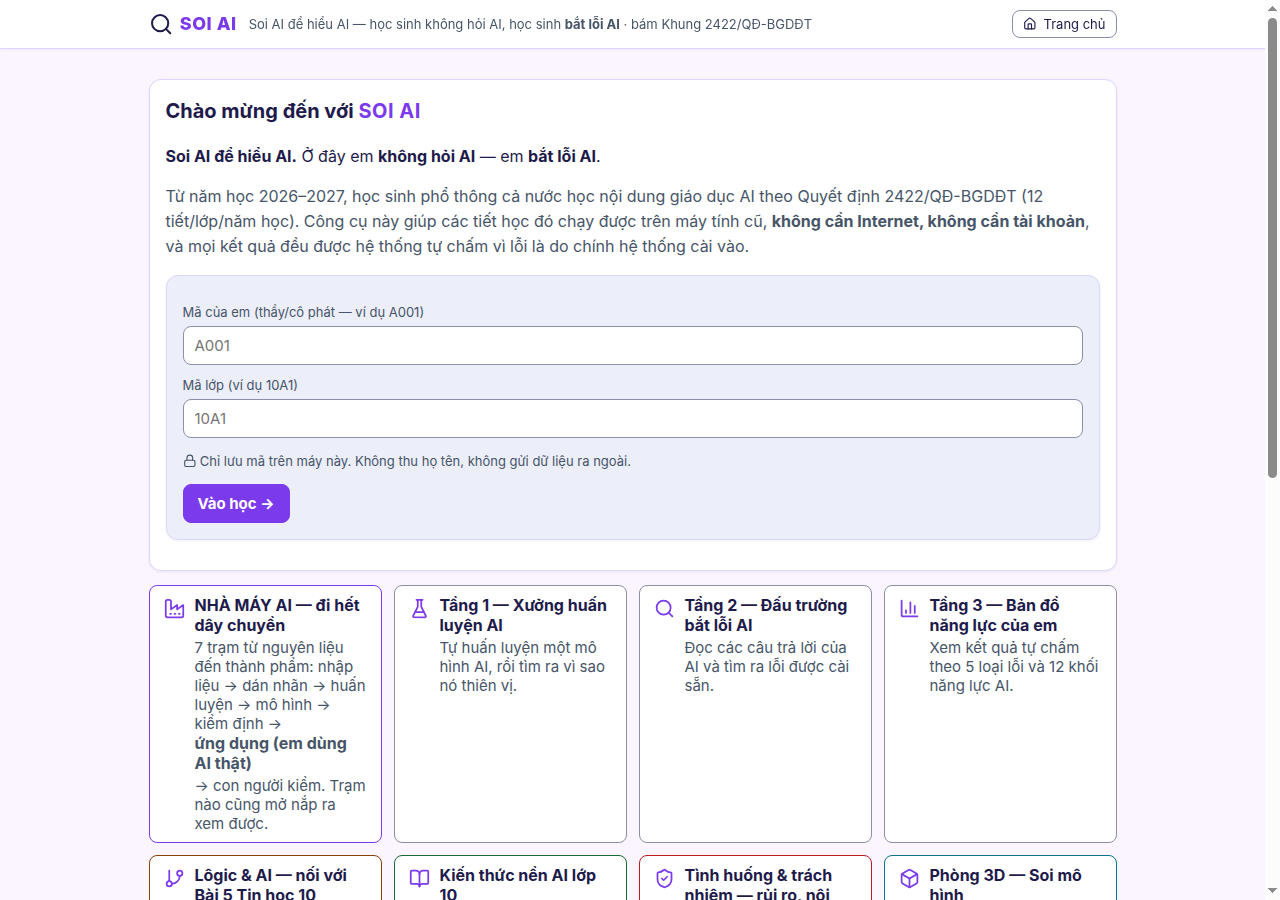
\includegraphics[height=4.05cm, keepaspectratio]{assets/1-trang-chu.png}
            \end{center}
        \end{block}
        \column{0.49\textwidth}
        \begin{block}{Nhà máy AI - 7 trạm}
            \begin{center}
                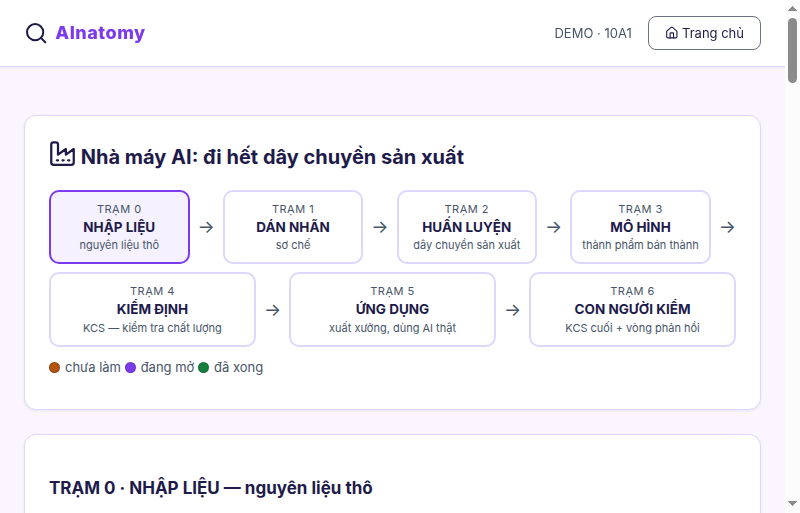
\includegraphics[height=4.05cm, keepaspectratio]{assets/2-nhamay-7tram.png}
            \end{center}
        \end{block}
    \end{columns}
    \vspace{0.3em}
    {\small Giao diện trực quan, dễ sử dụng. Học sinh có thể điều hướng qua các tầng và trạm.}
\end{frame}

\begin{frame}{4.3. Slider nội suy điều kiện sáng}
    \begin{columns}[t]
        \column{0.49\textwidth}
        \begin{block}{Tính năng}
            \begin{itemize}
                \item Slider trượt liên tục từ 0\% đến 100\%
                \item Nội suy màu sắc mượt mà: đêm $\rightarrow$ hoàng hôn $\rightarrow$ ngày
                \item Học sinh tự khám phá thiên kiến dữ liệu
            \end{itemize}
        \end{block}
        \column{0.49\textwidth}
        \begin{block}{Minh họa}
            \begin{center}
                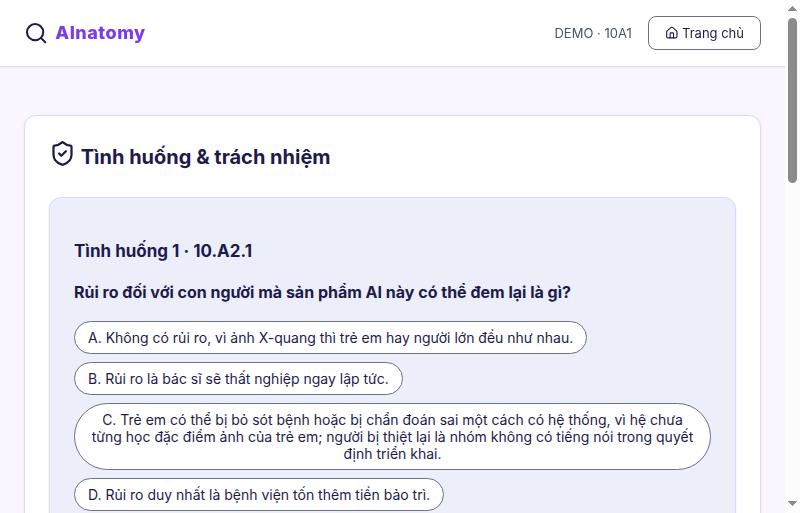
\includegraphics[height=3.5cm, keepaspectratio]{assets/3-slider-noisuy.png}
            \end{center}
        \end{block}
    \end{columns}
    \vspace{0.3em}
    {\small Khi kéo slider, học sinh quan sát 4 đặc trưng thay đổi theo điều kiện sáng, hiểu rõ nguồn gốc thiên kiến.}
\end{frame}

\begin{frame}{4.4. Tình huống đạo đức AI}
    \begin{columns}[t]
        \column{0.49\textwidth}
        \begin{block}{Tính năng}
            \begin{itemize}
                \item 12 tình huống thực tế về đạo đức AI
                \item Giao diện accordion, mỗi lần hiện 1 câu
                \item Phản hồi ngay sau khi chọn đáp án
            \end{itemize}
        \end{block}
        \column{0.49\textwidth}
        \begin{block}{Minh họa}
            \begin{center}
                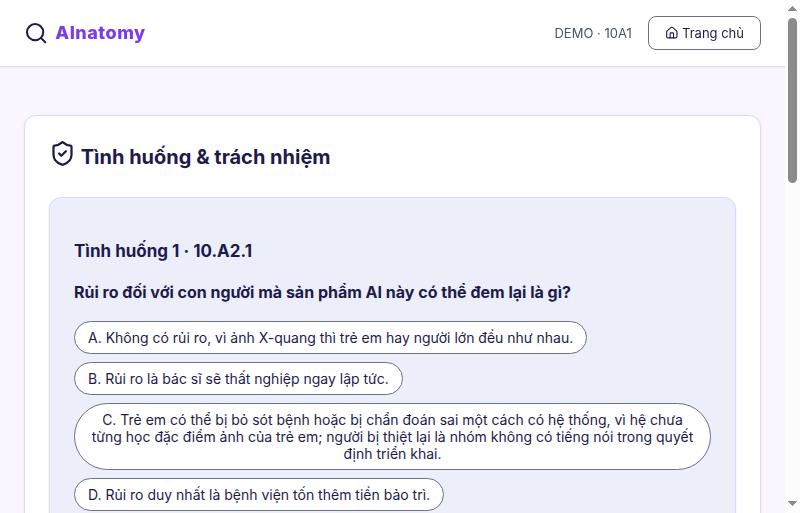
\includegraphics[height=3.5cm, keepaspectratio]{assets/4-tinhhuong-accordion.png}
            \end{center}
        \end{block}
    \end{columns}
    \vspace{0.3em}
    {\small Chủ đề: thiên kiến dữ liệu, quyền riêng tư, trách nhiệm khi AI sai, minh bạch thuật toán.}
\end{frame}

% ================= PHẦN 5: TÍNH BỀN VỮNG VÀ KHẢ NĂNG MỞ RỘNG =================
\section{Tính bền vững và khả năng mở rộng}

\begin{frame}{5. Tính bền vững và khả năng mở rộng}
    % Gộp 5.1 + 5.2 thành 1 slide để giữ giới hạn 15 trang sau khi thêm slide 4.2.
    \begin{columns}
        \column{0.5\textwidth}
        \begin{block}{Tính bền vững}
            \begin{itemize}
                \item Chạy offline, không phụ thuộc internet hay cloud.
                \item Mã nguồn mở, dễ bảo trì và cập nhật qua JSON.
                \item Không phụ thuộc nhà phát triển ban đầu.
            \end{itemize}
        \end{block}
        \column{0.5\textwidth}
        \begin{block}{Khả năng mở rộng}
            \begin{itemize}
                \item Mọi trường THPT có thể triển khai ngay.
                \item Mở rộng sang khối 11, 12 và chủ đề AI nâng cao.
                \item Tích hợp với các công cụ AI thực tế (ChatGPT, Gemini).
            \end{itemize}
        \end{block}
    \end{columns}
    
    \vspace{0.5em}
    
    \begin{block}{Tiềm năng dài hạn}
        \begin{itemize}
            \item Xây dựng cộng đồng giáo viên chia sẻ tài nguyên AInatomy.
            \item Nghiên cứu tác động dài hạn đến năng lực số học sinh.
            \item Đóng góp vào mục tiêu giáo dục AI quốc gia (QĐ 2422).
        \end{itemize}
    \end{block}
\end{frame}

% ================= KẾT LUẬN =================
\begin{frame}{Kết luận}
    \begin{itemize}
        \item AInatomy là phòng thí nghiệm AI offline, phủ 22/22 YCCĐ Tin học 10.
        \item Chạy hoàn toàn offline, phù hợp với điều kiện hạ tầng trường THPT Việt Nam.
        \item Giúp học sinh phát triển năng lực kiểm chứng AI: quan sát quy trình, dự đoán đầu ra, phát hiện lỗi, đánh giá độ tin cậy.
        \item Thiết kế module, dễ mở rộng cho khối 11, 12 và các chủ đề AI nâng cao.
    \end{itemize}
    
    \vspace{0.5em}
    
    \centering
    \textbf{Trải nghiệm AInatomy:} https://mxuanvan02.github.io/ainatomy/
\end{frame}

\begin{frame}{Kiến nghị}
    \begin{enumerate}
        \item \textbf{Bộ GD\&ĐT:} Khuyến khích các trường triển khai công cụ AI offline như AInatomy, đặc biệt ở vùng khó khăn.
        \item \textbf{Trường THPT:} Tích hợp AInatomy vào bài giảng Tin học 10, tổ chức tập huấn giáo viên về phương pháp dạy AI kiểm chứng.
        \item \textbf{Giáo viên:} Sử dụng AInatomy làm công cụ hỗ trợ giảng dạy, khuyến khích học sinh chất vấn AI thay vì tin tuyệt đối.
        \item \textbf{Nghiên cứu tiếp theo:} Mở rộng đánh giá tác động dài hạn của AInatomy đến năng lực số học sinh, phát triển thêm bài học cho khối 11, 12.
    \end{enumerate}
\end{frame}

\begin{frame}{Tài liệu tham khảo}
    \small
    \begin{enumerate}
        \item Bộ Giáo dục và Đào tạo (2018). \textit{Chương trình giáo dục phổ thông -- Môn Tin học}. Hà Nội.
        \item Bộ Giáo dục và Đào tạo (2024). \textit{Quyết định 2422/QĐ-BGDĐT về việc ban hành Khung nội dung giáo dục về trí tuệ nhân tạo trong các cơ sở giáo dục}. Hà Nội.
    \end{enumerate}
    % 3 tài liệu cũ (Nguyen & Le 2023; Smith & Johnson 2024; Tran 2025) đã bị xoá
    % sau khi tra Crossref: không tồn tại, không kiểm chứng được, là nguồn dựng
    % — nếu giữ lại sẽ bị giám khảo RMIT phát hiện ngay. Giữ đúng 2 nguồn chính
    % thức của Bộ GD&ĐT, đủ để chứng minh bối cảnh.
\end{frame}

% --- Slide kết thúc ---
\begin{frame}[plain]
    \centering
    \vspace{1cm}
    
\includegraphics[height=1.5cm, keepaspectratio]{logos/thpt_thuan_hoa} \hspace{2cm}
    
\includegraphics[height=1.5cm, keepaspectratio]{logos/dhsp_hue}
    
    \vspace{1.5cm}
    {\Huge \bfseries \color{HUEBlue} TRÂN TRỌNG CẢM ƠN!}\\
    \vspace{0.5cm}
    {\Large Q\&A}
\end{frame}

\end{document}
